% ---------------------------------------------------------------------------------------
\chapter{Prototipo funcional V1}\label{proto1}

Para continuar con el desarrollo del proyecto, se deben hacer funcionar las distintas partes (sensores, microcontrolador, módulo Bluetooth, Smartphone y servidor) como un todo y para ello se crea un primer hito de prototipado con el cual se espera alcanzar esta integración. Además de lo anterior, se espera poder hacer pruebas que asienten o desmientan decisiones de diseño y configuración, siempre con miras a los requerimientos generales del proyecto.

\section{Configuración final RN4020}

En el apartado del microcontrolador junto al módulo Bluetooth, se utiliza un archivo .ino con los parámetros necesarios y un ciclo de ejecución con el cual ofrecer la funcionalidad del envío de datos desde los sensores al Smartphone.

En esta primera configuración se hace uso de un Script para la configuración básica del chip RN4020 por parte del microcontrolador, se establece la visibilidad como activa desde el inicio de operación, se utilizan los parámetros por defecto al mínimo de conexión Bluetooth: Latencia (tiempo de respuesta), intervalo de conexión (frecuencia con que una comunicación es establecida), timeout(tiempo de espera antes de cancelar la comunicación) y se habilita la encriptación en la comunicación Bluetooth (AES-128, cirptografía simétrica).

Respecto a la comunicación entre el microcontrolador y el módulo se observa que los Baudios máximos se encuentran en los 19.200 [S/s], pasando por 2.400 [S/s] y 9.600 [S/s].\newpage


\section{Análisis de rendimiento por codificación }

En esta oportunidad se le da prioridad a la configuración del ECG por sobre los datos de temperatura, pese ya a tener configurada la característica asociada a ambos. Por lo que se realizan distintas pruebas modificando parámetros relevantes como la potencia (de transmisión del chip RN4020), la seguridad, cantidad de datos por envío y Baudios. Cabe mencionar que los datos deben ser convertidos a hexadecimal para ser entregados al módulo Bluetooth, por lo que se deben convertir tanto en el microcontrolador como en la aplicación móvil.

En la figura \ref{benchmark} se utilizaron:

\textbf{Distancia}:  Fija a 1 metro.

\textbf{Potencia}: Variable 4 y 7, a -2.5 [dBm] y 7.5 [dBm] respectivamente.

\textbf{Seguridad}: Enlazado y no enlazado.

\textbf{Línea vista}: No.

\textbf{Datos}: Hexadecimal de 1 [byte] representando enteros entre [0-255].


\begin{figure}[H]
	\centering
	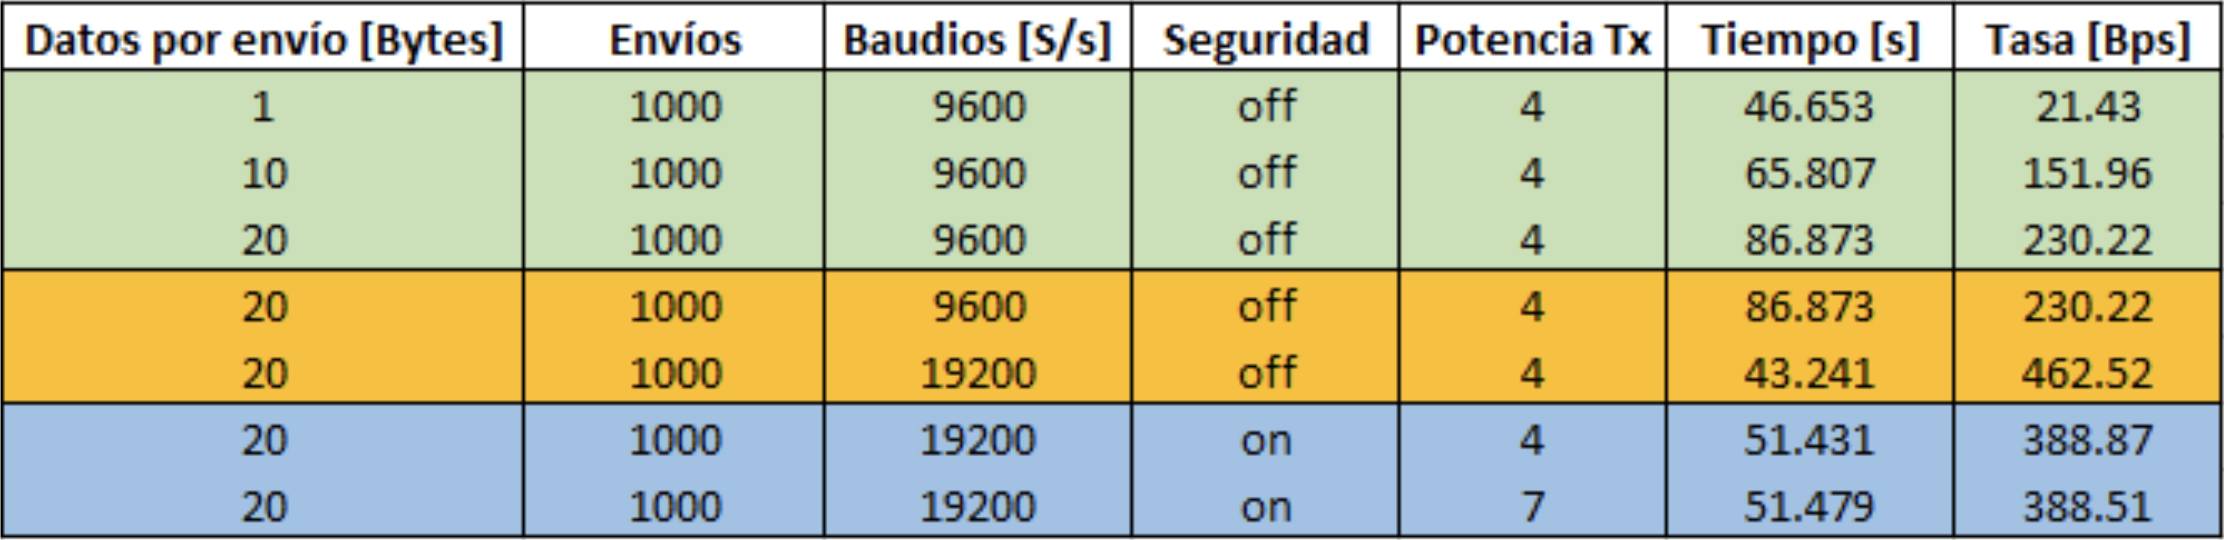
\includegraphics[scale=0.3]{figuras/proto1/benchmark.png}
	\caption{Resultados, pruebas de configuración ECG. Fuente: Elaboración propia}
	\label{benchmark}
\end{figure}

Con lo cual se justifica el uso de paquetes de 20 datos (máximo permitido en una misma instrucción por el módulo RN4020) por envío. Logrando así una frecuencia de al menos 200 [Bps] en el envío de datos si fuere necesario.
Además, se destaca que la seguridad no afecta significativamente y dada la distancia, la potencia de transmisión tampoco. Pese a lo anterior se baraja la posibilidad de usar una resolución de 10 bits (resolución máxima del sensor) a través del uso de 2 bytes hexadecimales, alcanzando un máximo de 10 datos por envío.

\section{Elementos en Android}

Luego de haber obtenido la base de aplicación en función del ejemplo en la página oficial de Microchip, la cual entrega las herramientas para comnunciarse con el chip RN4020, se busca dar forma a una aplicación que cumpla con las características del proyecto y que por el momento sea funcional en torno a lo obtenido hasta el momento.

Android es un SO ampliamente utilizado y por ende posee una gran comunidad a sus espaldas, las cuales frecuentemente otorgan librerías y mejoras constantes además de su propio responsable (Google). Con lo anterior en mente, se hace la búsqueda de distintas herramientas capaces de ofrecer funcionalidad y flexibilidad al proyecto, las cuales se describirán brevemente en conjunto con una explicación de por qué su uso frente a otras alternativas (no necesariamente mencionadas). Cabe destacar que el presente documento se hace al año 2018 y por ende con las capacidades actuales presentes en el desarrollo de una aplicación Android.\newline

\begin{figure}[H]
	\centering
	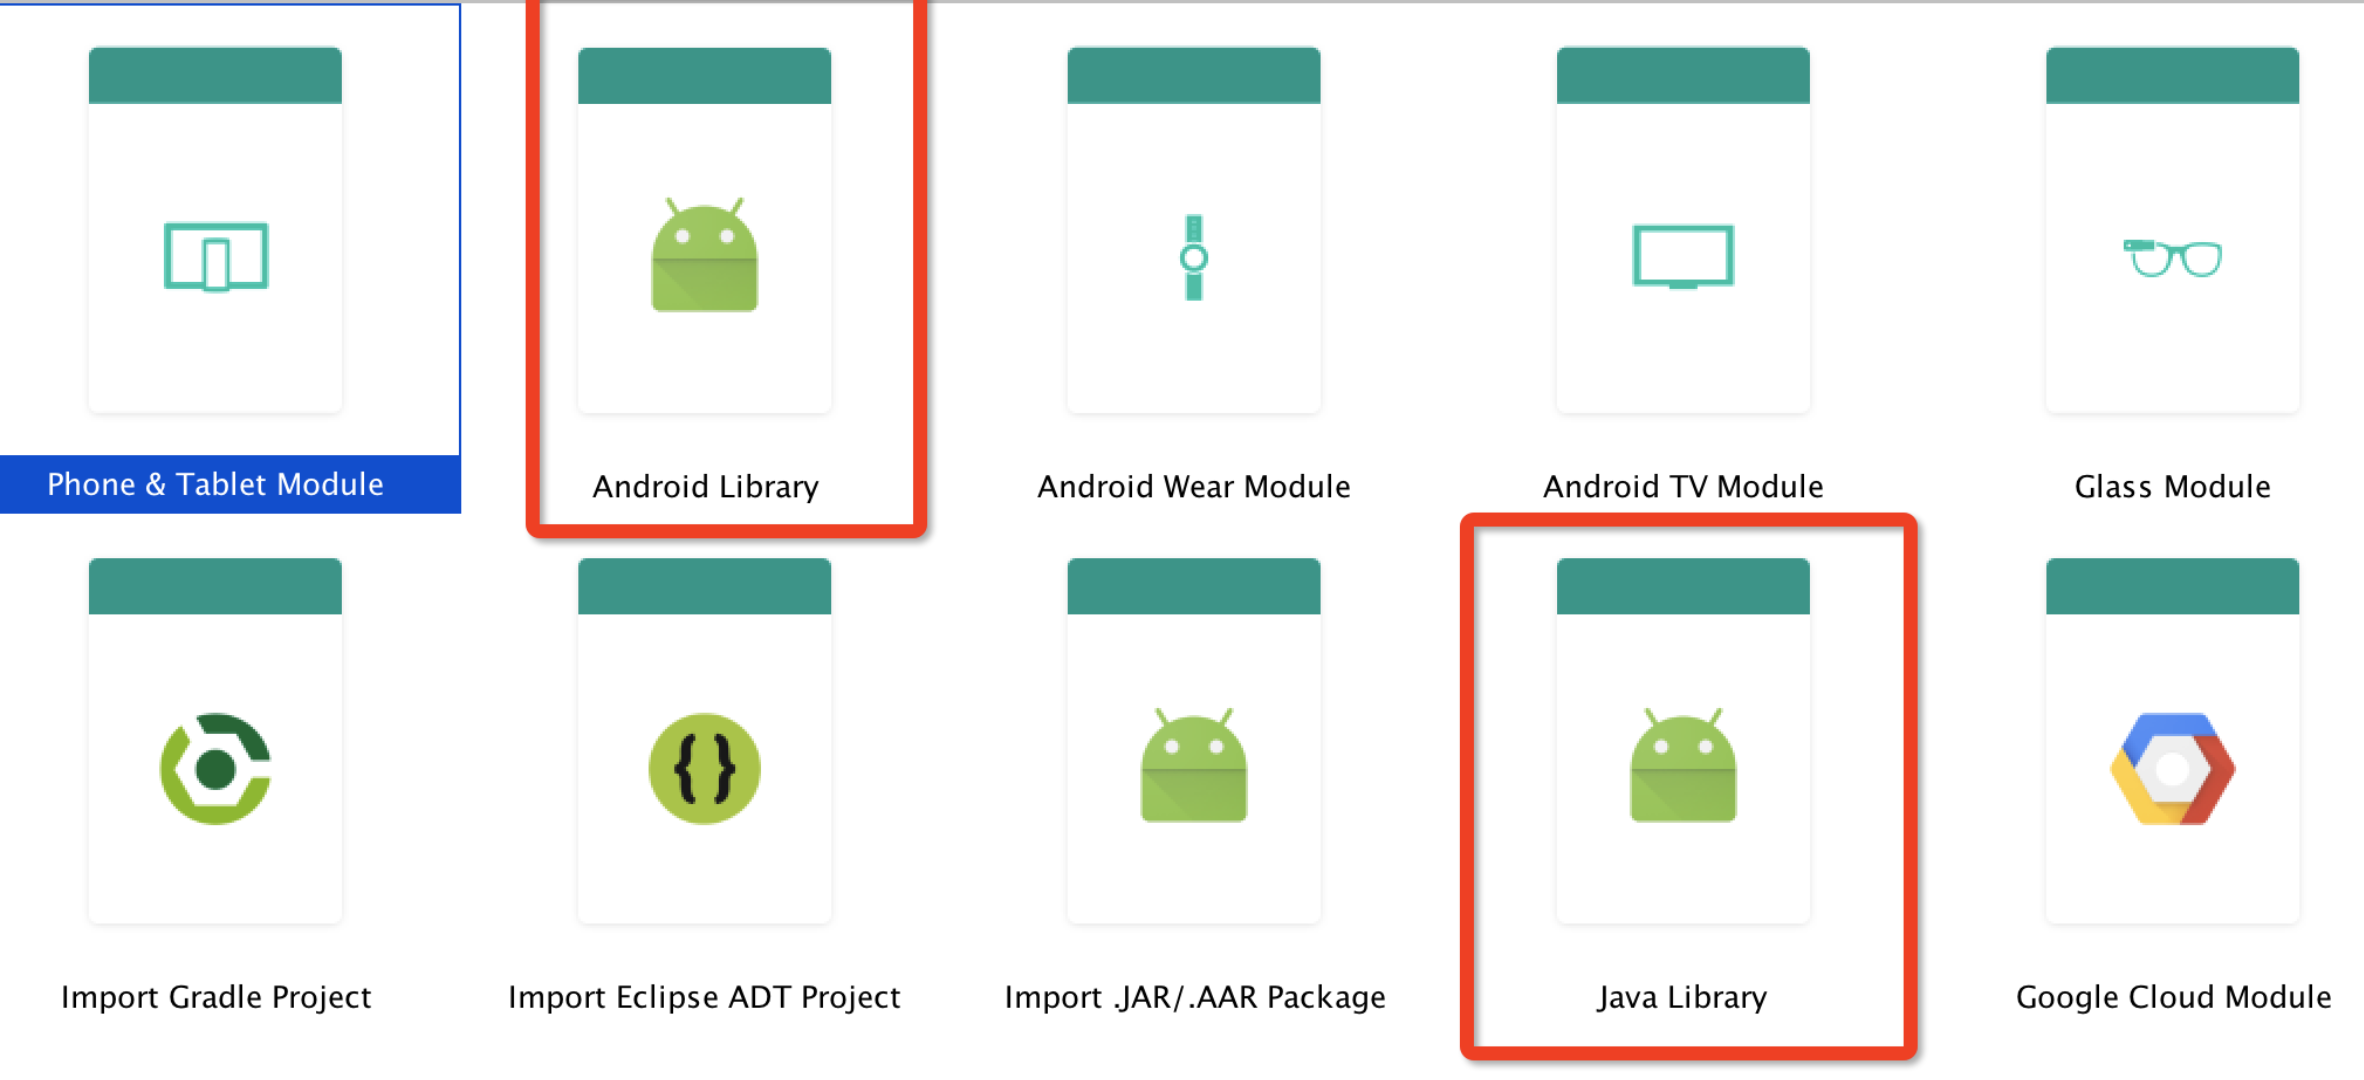
\includegraphics[scale=0.3]{figuras/proto1/library.png}
	\caption{Uso de librerías en Android. Fuente: Android Studio}
	\label{library}
\end{figure}

 \newpage

\subsection{RecyclerView}

En Android, existen diversas formas de generar visualmente listas para los usuarios, pero actualmente gracias a Google se cuenta con algo llamado RecyclerView. La cual funciona como contenedor de una lista como cualquier otra, pero pensada en el alto rendimiento (gran cantidad de elementos) y una estética cuidada en la fluidez de la misma. 

Para una aplicación como la presente no se hace necesario el uso de esta librería, dado que no se tiene una gran cantidad de elementos que desplegar en pantalla, pero siempre es bienvenida la velocidad de codificación que proporciona al presentar una arquitectura de plantillas sobre las cuales generar elementos. Así, es utilizada en el proyecto actual para contener distintos tipos de conexión  con su respectivo estado: Al servidor, con el módulo Bluetooth, y con el servicio propio de la aplicación.\newline

\begin{figure}[H]
	\centering
	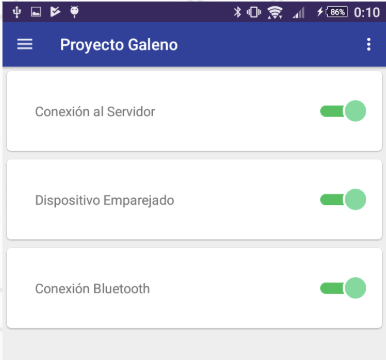
\includegraphics[scale=1]{figuras/proto1/recycler.png}
	\caption{Uso de RecyclerView. Fuente: Elaboración propia}
	\label{recycler}
\end{figure} 

\newpage

\subsection{Códigos QR}

Dado que el proyecto utiliza un emparejamiento con un dispositivo Bluetooth, es importante recordar que para lograr esto existen distintas técnicas, entre las que destacan el escaneo (alto consumo de potencia, lento y engorroso si existen diversos dispositivos), ingreso manual de la dirección física MAC del dispositivo al cual conectarse (lento y engorroso) y por ingreso automático (utilizando la cámara como medio físico y alguna codificación ya establecida). Es en este último punto en donde los códigos de barra surgen como una opción rápida y cómoda, más aún cuando se utiliza a los códigos QR, los cuales estandarizan la codificación básica de cualquier cadena de texto. Otorgando así comúnmente direcciones URL, de las cuales se obtienen diversos recursos (imágenes, video, texto, entre otros).

Es por lo anterior que se decide emplear a los códigos QR como la forma más efectiva de entregar la dirección física de los módulos Bluetooth, con la cual la aplicación podrá efectuar el emparejamiento respectivo.

Para esta acción existen diversas librerísa disponibles, pero de entre ellas se destaca a ZXING, la cual ofrece tanto la creación como la lectura de distintos tipos de códigos. Hace unos años esta librería solo podía usarse en conjunto con una aplicación, pero actualmente es posible encontrarla por separado: QRCodeReaderView es una versión modificada de ZXING que permite leer códigos QR de forma simple y rápida (aunque con pocas opciones de personalización de interfaz).

\begin{figure}[H]
	\centering
	
\includegraphics[scale=0.6]{figuras/proto1/qr.png}
	\caption{QR con MAC de dispositivo Bluetooth. Fuente: Elaboración propia}
	\label{qr}
\end{figure}

\subsection{Fragment}

Este es un elemento básico en Android y es utilizado como una versión menor de las Activitys, es utilizado comúnmente como contenedor de vistas menores y controlados en conjunto por una Activity.
Su uso en el proyecto fue decidido por el menú lateral escogido para albergar las distintas vistas de la aplicación.

\begin{figure}[H]
	\centering
	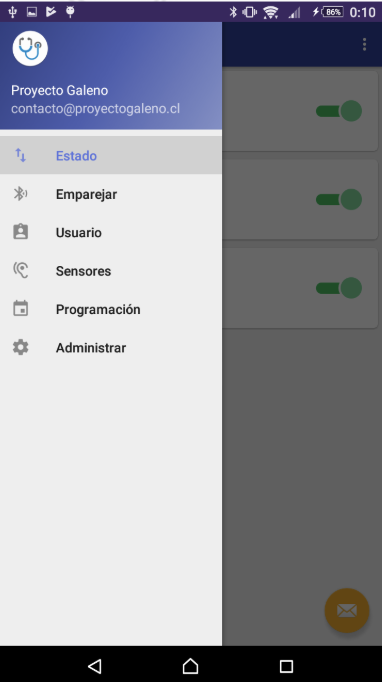
\includegraphics[scale=1]{figuras/proto1/fragment.png}
	\caption{Menú lateral comprendido por distintos Fragment. Fuente: Elaboración propia}
	\label{fragment}
\end{figure}

Si bien no todas esas vistas fueron implementadas (Usuario y Programación) en este punto, se tuvo claridad de las mismas desde un inicio y se tuvo consideración en la facilidad de uso, agrupando las opciones según función.

\subsection{MPAndroidChart}

La visualización es una funcionalidad necesaria con el fin de validar pruebas y otorgar al mismo tiempo un prototipo con mayor solidez hacia la contraparte. Es por esta razón que se analizaron distintas opciones de librerías, dentro de las cuales destacó MPAndroidChart, librería nativa de Android, con gran rendimiento y opciones de personalización. Es sencilla de utilizar y ofrece la posibilidad de gráficos en tiempo real, dependiendo del dispositivo se pudieron obtener sobre 1000 puntos al mismo tiempo con gran fluidez, algo realmente importante si se considera que el ECG posee un gran flujo de datos (típicamente de 50 [Hz] - 150 [Hz]).

\begin{figure}[H]
	\centering
	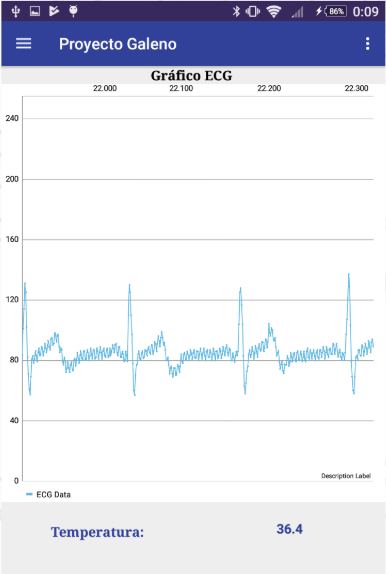
\includegraphics[scale=1]{figuras/proto1/graph.png}
	\caption{Gráfico en tiempo real con datos de ECG por Bluetooth. Fuente: Elaboración propia}
	\label{graph}
\end{figure}

Como se puede observar en la figura \ref{graph}, se observa gran cantidad de ruido, aspecto corregido hasta cierto punto en posteriores iteraciones.

\subsection{Shared Preference}

El proyecto requiere que la dirección MAC sea almacenada en alguna memoria persistente con el fin de poder reconectar los dispositivos de ser necesario: Al apagar el Smartphone o el Arduino, al aumentar demasiado la distancia, entre otros. La dirección MAC no es otra cosa que una cadena de texto, por lo que un almacenamiento básico es suficiente para los objetivos del proyecto.

Por lo anterior se decanta por la utilización de Shared Preference (Preferencias compartidas) como el método de almacenamiento, esta es una característica que ofrece Android de forma base, la cual permite por aplicación un almacenamiento tipo llave-valor, estilo diccionario. La cual es accesible solo desde la misma aplicación o compartida entre distintas aplicaciones, pero con persistencia al cierre de las mismas (lo que realmente es fundamental para el proyecto).

\subsection{Inicio automático de Servicio y otros}

En esta sección se detallará un poco más sobre los elementos del menú y el  comportamiento del primer prototipo del proyecto:

\textbf{Estado}: RecyclerView con distinto estados de conexión (Servidor, BT y Servicio).

\textbf{Emparejar}: Lector de códigos QR para asociar MAC de un dispositivo.

\textbf{Sensores}: Presentación visual de los datos recibidos en tiempo real.

\textbf{Usuario}: Datos almacenados en Android del paciente (aún sin implementar).

\textbf{Programación}: Futura mejora para mostrar próximas tomas de datos.

\textbf{Administración}: Manejo del estado del servicio principal.

Respecto a su comportamiento, se establece por medio del Manifest (archivo de cada proyecto en Android que controla permisos, articula las distintas Activity y ciertos parámetros generales) la apertura del servicio al arranaque del SO, mientras el servicio se encuentre activo se encarga de mantener encendido el adaptador Bluetooth del Smartphone y se utiliza la opción de enlazado provisto por el SO Android (por fuera de la aplicación y mencionado al final del capítulo 8).
 

